{
\abnormalparskip{0pt}
\chapter{Experiments}
\label{cha:experiments}
}

This chapter describes and discusses the experiments that have been performed in
relation to the new implementation.

All experiments have been executed on computer with $8 \times$
Intel\textsuperscript{\textregistered} Xeon\textsuperscript{\textregistered} CPU
E5-2630L at $2.00$ GHz and with $16$ GB RAM. Furthermore all tests were executed
using version $1.4.2$ of Go\footnote{A newer version (1.5) which improves the performance of
  the language due to more efficient garbage collection was released after the
  experiments had been conducted.}. In the experiments the used methods are
named as seen in \cref{tab:method-names}.

\begin{table}[htbp]
  \centering
  \begin{tabular}{cp{9cm}}
    \toprule
    Method                & Description                                                                                                                                      \\
    \midrule
    \texttt{Simple}       & New implementation using the analytical method. Implemented in Go.                                                                               \\
    \texttt{SimpleSort}   & New implementation using the analytical method and with terminal sorting. Implemented in Go.                                                     \\
    \texttt{SmithNew}     & New implementation using \citeauthor{smith1992}'s iteration. Implemented in Go.                                                                  \\
    \texttt{SmithNewSort} & New implementation using \citeauthor{smith1992}'s iteration and with terminal sorting. Implemented in Go.                                        \\
    \texttt{SmithOld}     & Original implementation by \textcite{smith1992}, only slightly modified to fix the bug described in \cref{sec:if-clause-when}. Implemented in C. \\
    \bottomrule
  \end{tabular}
  \caption[Naming of methods]{The naming of methods has been done in the
    experiments as shown here.\label{tab:method-names}}
\end{table}

In general the experiments performed, relates to either
correctness or performance of the implementation. The correctness has been
measured by comparing a set of instances with the results found by the
GeoSteiner program. The performance experiments is divided into experiments
regarding the speed of the methods, the number of trees which are optimized, and
the number of iterations being run. 

\section{Correctness}
\label{sec:correctness}

To test the correctness of the new implementation $150$ random cube instances
with $n = 10 \ldots 12$ and $d = 2$ has been run. The cube instances are the
same as used by \textcite{fonseca2014}, which can also be found at
\url{https://github.com/DIKU-Steiner/MPC15/tree/master/experiments/Correctness/Instances}.
The the terminals of the instances are randomly distributed in a unit cube.

The experiments was run for all of the methods in \cref{tab:method-names},
except \texttt{SmithOld} which I had no interest in testing the correctness of,
as this has been done before. To compare the instances was also completed using
the official GeoSteiner implementation\footnote{The implementation can be found
  at downloaded at \url{http://geosteiner.com}}.

After all instances were completed, the results of the new implementation were compared
with the results of the GeoSteiner program. This showed that analytical solution,
both with and without terminals sorting, in a few instances gave sub-optimal
\acp{smt}. These and the difference to the optimal \ac{smt} found by GeoSteiner
can be found in \cref{tab:correctness-errors}.

\begin{table}[htbp]
  \centering
  \begin{tabular}{ccc}
    \toprule
    Instance           & Method              & Diff       \\
    \midrule
    cube\_n12\_d2\_s27 & \texttt{Simple}     & $+0.170\%$ \\
    cube\_n12\_d2\_s49 & \texttt{Simple}     & $+0.295\%$ \\
    cube\_n10\_d2\_s42 & \texttt{SimpleSort} & $+0.015\%$ \\
    cube\_n12\_d2\_s26 & \texttt{SimpleSort} & $+0.228\%$ \\
    cube\_n12\_d2\_s43 & \texttt{SimpleSort} & $+0.292\%$ \\
    cube\_n12\_d2\_s49 & \texttt{SimpleSort} & $+0.295\%$ \\
    \bottomrule
  \end{tabular}
  \caption[Sub-optimal results in correctness test]{The table shows the
    instances in which some method gave sub-optimal results, and the difference
    in percent to the optimal \acp{smt} found by the GeoSteiner
    program.\label{tab:correctness-errors}}
\end{table}

As can be seen \texttt{Simple} gave sub-optimal results in $2$ instances, and
\texttt{SimpleSort} in $4$ instances, meaning that $6$ of $300$ ($2\%$) instances
gave sub-optimal results. Neither \texttt{SmithNew} or \texttt{SmithNewSort}
gave any errors.

When inspecting the \acp{smt} generated by the simple method in the sub-optimal
instances, it was clear, that the method in these case indeed gave different
topologies from the topology found by the GeoSteiner program.

The reason for this, I believe can be traced back to two things: the two
if-clauses in the implementation used when optimizing, and the possibility that
the error function defined by \citeauthor{smith1992} is faulty.

\begin{figure}[htbp]
  \begin{c-code}
    ITER:
    q = length();
    r = error();
    if ( q - r < STUB) {
      if (r > 0.005*q) {
        optimize(0.0001*r/NUMSITES);
        goto ITER;
      }
      /* Truncated code.
         Pushes topology and length to stack.
         Continue working with the topology and its descendants */
    }
    /* Continue to next topology vector of same length,
       if we have no been in the outer if-clause then all
       descendants of the current topology vector is 
       effectively pruned as we have not stored it on the stack. */
  \end{c-code}
  \captionof{listing}[Loop condition for pruning topologies]{The outer if-clause
    decides whether we prune a topology or not. This is applied before the
    topology is optimized to its \acs{rmt}, which significantly speeds up the
    program. But whether this is allowed is unclear. The code snippet is from
    \autocite{smith1992}'s implementation, given in~\cite{smith1992}. The new
    implementation in Go uses the same two
    conditions.\label{fig:loop-condition-pruning}}
\end{figure}

Consider the the code snippet in \cref{fig:loop-condition-pruning}, which is
from the original implementation found in \textcite{smith1992}. What happens in
the snippet is the following: before any optimization iterations has taken
place, the length and error of the tree is calculated. A check (the first if-clause) whether the
length minus the error is lower than the upper bound ($q-r < \textit{STUB}$)
is then performed. If the check is yields false, the main loop continues without
pushing the topology vector to the stack used described
in \cref{sec:order-build-optim}. This means that any descendant of that topology
vector will not be optimized, i.e.\ they are pruned. If the check yields true,
the the program goes to the second if-clause which checks if the error is
greater than $0.005 \cdot q$. If the second check yields true, the tree is
optimized, and the program return to the \texttt{ITER} label. If it yields
false, the program continues on, within the first if-clause, and eventually push
the topology vector to the stack.

The structure just described means that we can both discard a topology before
optimizing it, or after optimizing some for some number of iterations. This
significantly speeds up the program, in contrast to optimizing the topology to
its \ac{rmt} and then deciding whether it must be pruned or not. The new
implementation therefore retained this structure.

However as described in \cref{sec:loop-condition-when-1} there seems to be no
direct relation between the length and error of the tree. Also as described in
\cref{sec:choice-error-funct} it is even unclear whether the error function is
even correct. Thus both of these if-clauses are a bit sketchy.

\begin{figure}[htbp]
  \centering
  \begin{subfigure}[b]{0.4\textwidth}
    \includegraphics[width=\textwidth]{gfx/tikz/upperbound-2}
    \caption{Example where subtracting the error from the tree
      length yields a length shorter than the current upper bound. In this case
      the program would continue to to optimize on the topology, and there is no
      risk of prematurely pruning it.\label{fig:upperbound-2}}
  \end{subfigure}\hspace{1em}
  \begin{subfigure}[b]{0.4\textwidth}
    \includegraphics[width=\textwidth]{gfx/tikz/upperbound-1}
    \caption{Example where subtracting the error from the tree
      length yields a length greater than the current upper bound. If it is not
      always the case that $q-r \le \ac{rmt}$ then this situation could
      potentially result in a topology being pruned
      prematurely.\label{fig:upperbound-1}}
  \end{subfigure}
  \caption[Upper bounds, 1 and 2]{Here be dragons.\label{fig:upperbound-1-2}}
\end{figure}

Consider the first if-clause. This assumes that subtracting the current error
from the current tree length, will always yield something which is lower than or
equal to the \ac{rmt} of the topology. If this is not the case, then it could be
possible to get a tree which if optimized would be shorter than the current
upper bound, but where subtracting the current error from the current tree
length would not be shorter than the current upper bound. This could result in a
topology being thrown away even if it should have actually been kept. The two
situations are shown in \cref{fig:upperbound-2-3}.

To test the impact of the first if-clause the instances were run again where the
condition of the first if-clause was changed to $q - 10 \cdot r <
\textit{STUB}$. The observed result that some of the instances which before gave
sub-optimal results were solved to optimality, while other new ones gave
sub-optimal results. These can be seen in \cref{tab:correctness-errors-4}. As
can be seen \texttt{Simple} and \texttt{SimpleSort} were still the only methods
to give sub-optimal results.

\begin{table}[htbp]
  \centering
  \begin{tabular}{ccc}
    \toprule
    Instance           & Method              & Diff       \\
    \midrule
    cube\_n11\_d2\_s9  & \texttt{SimpleSort} & $+0.262\%$ \\
    cube\_n12\_d2\_s12 & \texttt{Simple}     & $+1.405\%$ \\
    cube\_n12\_d2\_s43 & \texttt{SimpleSort} & $+0.292\%$ \\
    cube\_n12\_d2\_s9  & \texttt{SimpleSort} & $+0.214\%$ \\
    \bottomrule
  \end{tabular}
  \caption[Sub-optimal results with condition $q - 10 \cdot r < \textit{STUB}$]{
    Changing the condition of the first if-clause to $q - 10 \cdot r <
    \textit{STUB}$ causes the number of sub-optimal results drop to $4$.
    However some of these are were not sub-optimal before the
    change.\label{tab:correctness-errors-4}}
\end{table}

The instances which were not solved optimally before, but were after the change
seems to indicate that this condition indeed is partly to blame for the
sub-optimality. The reason that new instances suddenly gave sub-optimal results
I believe is because these instances now explore topologies which they before
would have discarded.

Now consider the second if-clause. This assumes two things, firstly that size of
the error is proportional to the length of the tree, and secondly that the error
of the entire tree represents the optimality of the entire tree. The first
assumption does have some merit. If one looks at the error function, as it is
defined in \cref{eq:28} it is clear, that if we have longer edges, they will
contribute more than shorter edges. Whether there is a direct relation between
error and length is however still unclear. The second assumption however faces
some problems in the new implementation. This assumes that we will not hit a
a situation in which most of the tree is optimal, but e.g.\ a single Steiner
point contributes a large error and is at a sub-optimal placement. This is a
problem, as a single Steiner point at a wrong position can propagate changes
throughout the tree when it is optimized. It may therefore be, that the tree is
not at all optimal, and that we therefore risk stopping prematurely.

\begin{table}[htbp]
  \centering
  \begin{tabular}{ccc}
    \toprule
    Instance           & Method              & Diff       \\
    \midrule
    cube\_n12\_d2\_s27 & \texttt{Simple}     & $+0.170\%$ \\
    cube\_n12\_d2\_s49 & \texttt{Simple}     & $+0.295\%$ \\
    cube\_n10\_d2\_s42 & \texttt{SimpleSort} & $+0.015\%$ \\
    cube\_n12\_d2\_s26 & \texttt{SimpleSort} & $+0.228\%$ \\
    cube\_n12\_d2\_s38 & \texttt{SimpleSort} & $+0.071\%$ \\
    cube\_n12\_d2\_s43 & \texttt{SimpleSort} & $+0.291\%$ \\
    cube\_n12\_d2\_s49 & \texttt{SimpleSort} & $+0.295\%$ \\
    \bottomrule
  \end{tabular}
  \caption[Sub-optimal results with condition $r > 0.0005 \cdot q$]{Changing
    the condition of the second if-clause to $r > 0.0005 \cdot q$ causes the
    number of sub-optimal results increase to $7$.\label{tab:correctness-errors-2}}
\end{table}

This may not have been a problem in the old implementation which rebuilt the
topology every time it was changed, however the new implementation does not
rebuild the entire topology, but reuses the already found placements when
splitting the topology. Thus the issue might be magnified by this new approach. 

A question which of course emerges, is why the issue with sub-optimality is seen
then only seen with \texttt{Simple} and \texttt{SimpleSort} but not with
\texttt{SmithNew} and \texttt{SmithNewSort}. I.e.\ why does the analytical
solution show this issue, but not \citeauthor{smith1992}'s iteration?

The reason for this, I believe, is that the analytical solution when it runs, in
general obtains much lower error-figures than \citeauthor{smith1992}'s
iteration. I therefore believe that the issue exists for both iteration methods,
but is magnified and therefore only seen when using the analytical solution.

The potential problem is summed up by \cref{fig:upperbound-5}. We may have some
topology which has been optimized to have a very low error, this is particularly
likely using the analytical solution which attains very low error-figures. Upon
splitting the topology and adding the next terminal and a new Steiner point, the
error is raised. However because the error of the rest of the is very low,  

\begin{figure}[htbp]
  \centering
  \begin{subfigure}[b]{0.4\textwidth}
    \includegraphics[width=\textwidth]{gfx/tikz/upperbound-3}
    \caption{here be dragons.\label{fig:upperbound-3}}
  \end{subfigure}\hspace{1em}
  \begin{subfigure}[b]{0.4\textwidth}
    \includegraphics[width=\textwidth]{gfx/tikz/upperbound-4}
    \caption{here be dragons.\label{fig:upperbound-4}}
  \end{subfigure}
  \caption[Upper bounds, 3 and 4]{Here be dragons.\label{fig:upperbound-3-4}}
\end{figure}

\begin{figure}[htbp]
  \centering
  \includegraphics[width=.4\textwidth]{gfx/tikz/upperbound-5}
  \caption[Upper bounds, 5]{here be dragons.\label{fig:upperbound-5}}
\end{figure}

To test the impact of the second if-clause the instances were run with the
condition of the clause change to $r > 0.05 \cdot q$ and $r > 0.0005 \cdot q$.
The sub-optimal results from these runs can be found in
\cref{tab:tab-correctness-2,tab:tab-correctness-3}. As can be seen, allowing a
higher error gives fewer sub-optimal results, whereas setting the error even
lower raises the number of sub-optimal instances produced by the analytical
solution.

\begin{table}[htbp]
  \centering
  \begin{tabular}{ccc}
    \toprule
    Instance           & Method              & Diff       \\
    \midrule
    cube\_n12\_d2\_s27 & \texttt{Simple}     & $+0.170\%$ \\
    cube\_n12\_d2\_s43 & \texttt{SimpleSort} & $+0.292\%$ \\
    \bottomrule
  \end{tabular}
  \caption[Sub-optimal results with condition $r > 0.05 \cdot q$]{Changing
    the condition of the second if-clause to $r > 0.05 \cdot q$ causes the
    number of sub-optimal results drop to $2$.\label{tab:correctness-errors-3}}
\end{table}

These observations make seems to align with the before described problems.
Consider setting allowing a higher error. \TODO{}

Further raising the error allowed in the second if-clause to $r > 0.5 \cdot q$
resulted in sub-optimal results being observed across all four of the tested
methods. This is due to the fact the we at this point have raised the error so
much that the optimal trees cannot be obtained in all situations. This also
shows that we cannot simply raise the allowed error for the entire tree to
ensure we will not get sub-optimal results, as it will have to walk a tightrope
between sub-optimality due to to high errors, or sub-optimality due to the
previous described issues.

To correct this problem I believe one would have to do two things. Firstly,
before deciding whether to prune a topology and its descendants one would have
to optimize the tree until it was the \ac{rmt}, i.e.\ drop the condition $q-r <
\textit{STUB}$, and instead optimize until we have the \ac{rmt} and then simply
check $q < \textit{STUB}$, or perhaps $q - \epsilon < \textit{STUB}$ where
$\epsilon$ would be some very small positive number. This would prevent pruning
of topologies prematurely. Secondly, at least when using the analytical solution
(\textit{Simple} and \textit{SimpleSort}) the second if-clause should not look
at the error of the entire tree, but instead at the error of each individual
Steiner point. This would prevent the situation where most of tree has an error
of zero, and one point contributes most of the error. This approach might also
be the correct one for \textit{SmithNew} and \textit{SmithNewSort} as they also, in
contrast to \textit{SmithOld}, do not re-position the already placed Steiner
points when splitting the topology (due to the new method were we can split and
restore a topology, in contrast to the old method where one had to rebuild the
tree from the topology vector every time it was changed).

As the issue was first discovered during the experiments, the current
implementation does not fix it. I however believe this could be done using the
changes described above. It is however unclear how much this would affect the
run-time of the program.

However I do not believe it invalidates the performance data completely, as the
number of sub-optimal trees in the correctness test, was still very low, and the
sub-optimality of these trees also was relatively low.

\section{Performance}
\label{sec:performance}

To test the performance of the implementation the test sets in
\cref{tab:test-sets} has been run for all of the methods described in
\cref{tab:method-names}. All sets have been taken from \textcite{fonseca2014},
but the sets Carioca and Cube has been pruned. This has been done due to the
sheer size of these sets. Even with these sets pruned, running all of the sets
for all of the methods took a little more than a week in which a quad-core
computer ran 24/7. To further prune, all runs was set up such that they would
halt if more than $12$ hours passed, as it is then concluded infeasible to solve
that specific instance using the given method. How many instances completed
before the time limit can be seen in \cref{tab:set-success}.

A few initial test runs showed that, especially \texttt{SimpleSort} but also
occasionally \texttt{SmithNewSort}, were able to solve several instances with
$n=16$, and a few for $n=17$ within the $12$ time limit. Time-wise it was
however still infeasible to perform a proper test with these instance sizes.
Thus the new implementation solves instances about the same size as
\textcite{fonseca2014}.

\begin{table}[htbp]
  \centering
  \begin{tabular}{ccccc}
    \toprule
    Set     & Dimensions       & Terminals             & Set size & Point configuration \\
    \midrule
    Carioca & $d = 3 \ldots 5$ & $n = 11 \ldots 16$    & $90$     & Random in cube      \\
    Cube    & $d = 2 \ldots 4$ & $n = 10 \ldots 15$    & $360$    & Random in cube      \\
    Iowa05  & $d = 3 \ldots 5$ & $n = 10$              & $30$     & Random in cube      \\
    Sausage & $d = 2 \ldots 5$ & $n = 10 \ldots 15$    & $24$     & Simplex sequence    \\
    \bottomrule
  \end{tabular}
  \caption[Test sets used to test performance]{The table shows the tests sets,
    their dimensions, number of terminals, number of instances and type of instances,
    which has been used to test the performance of the implementation.\label{tab:test-sets}}
\end{table}

The data collected from the runs have been used to compare the speed (i.e.\
run-time), the number of iterations, and the number of trees optimized. The
results are presented and described in the two sections below.

\begin{table}[htbp]
  \centering
  \begin{tabular}{cccccc}
    \toprule
            & \multicolumn{5}{c}{Method}                             \\
    \cmidrule(l){2-6}
    Set     & \texttt{Simple} 
            & \texttt{SimpleSort}
            & \texttt{SmithNew} 
            & \texttt{SmithNewSort}
            & \texttt{SmithOld}                                      \\
    \cmidrule(r){1-1}\cmidrule(l){2-6}
    Carioca & $81/90$  & $89/90$  & $73/90$   & $87/90$  & $76/90$   \\
    Cube    & $\checkmark$ & $\checkmark$ & $352/360$ & $\checkmark$ & $356/360$ \\
    Iowa05  & $\checkmark$ & $\checkmark$ & $\checkmark$  & $\checkmark$ & $\checkmark$  \\
    Sausage & $22/24$  & $23/24$  & $18/24$   & $22/24$  & $21/24$   \\
    \bottomrule
  \end{tabular}
  \caption[Successfull test runs]{The table shows the number of successful
    instances, i.e.\ instances which finished within $12$ hours, of the test
    sets which has been run. A checkmark indicates all instances of the set was
    solved.\label{tab:set-success}}
\end{table}

\subsection{Speed}
\label{sec:speed}

\begin{figure}[htbp]
  \centering
  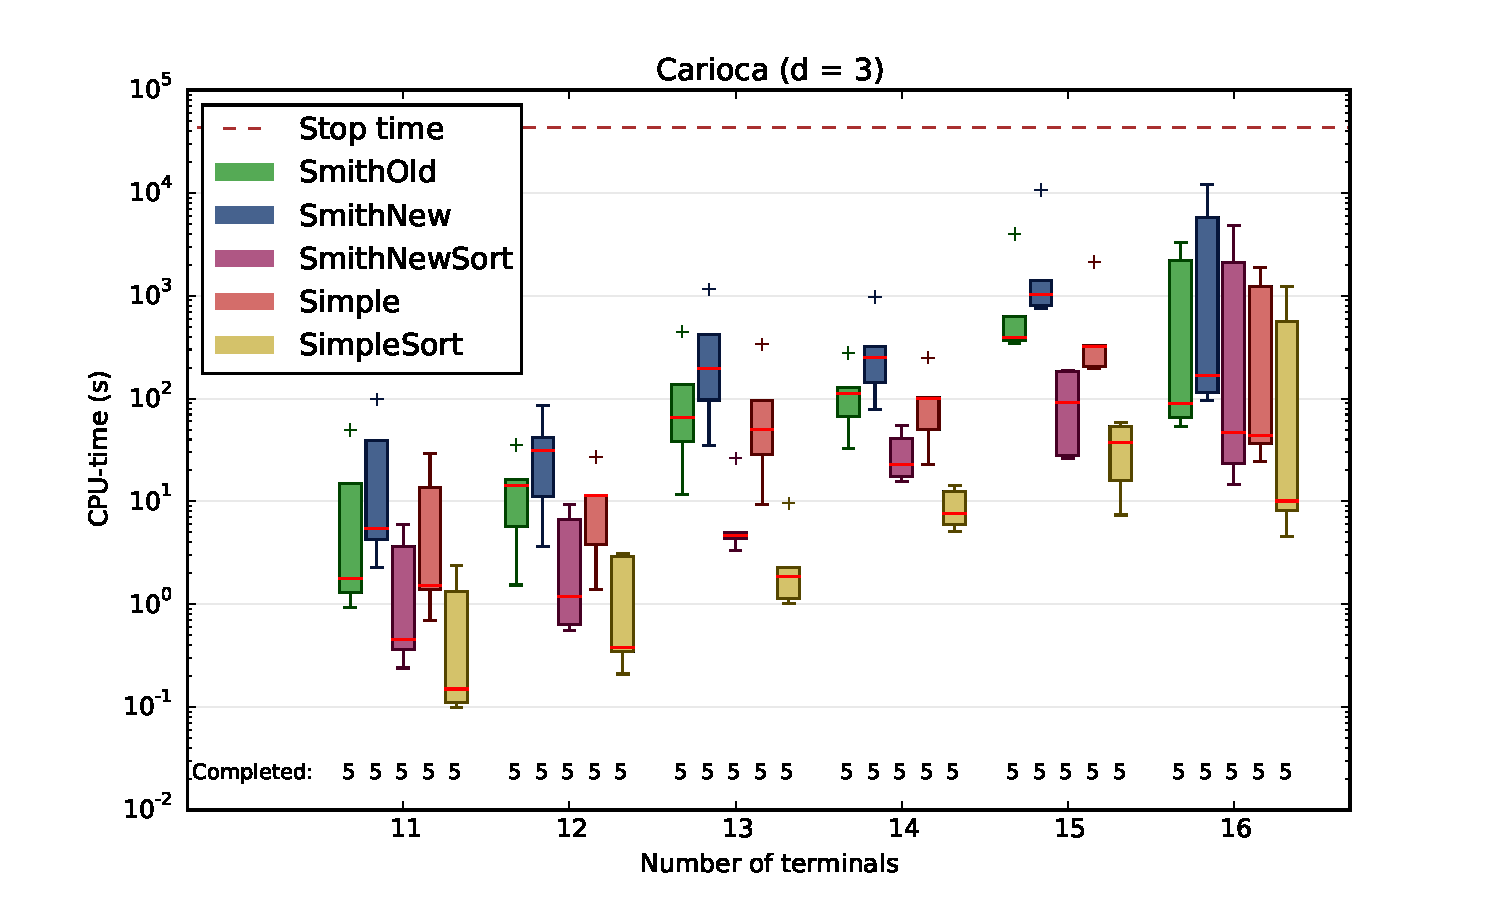
\includegraphics[width=0.8\textwidth]{gfx/boxplots/plot_nvst_boxplot_d3_Carioca_1}
  \caption[Box-plot for Carioca with $d = 3$]{Here be dragons.\label{fig:boxplot-carioca-d3}}
\end{figure}

\begin{figure}[htbp]
  \centering
  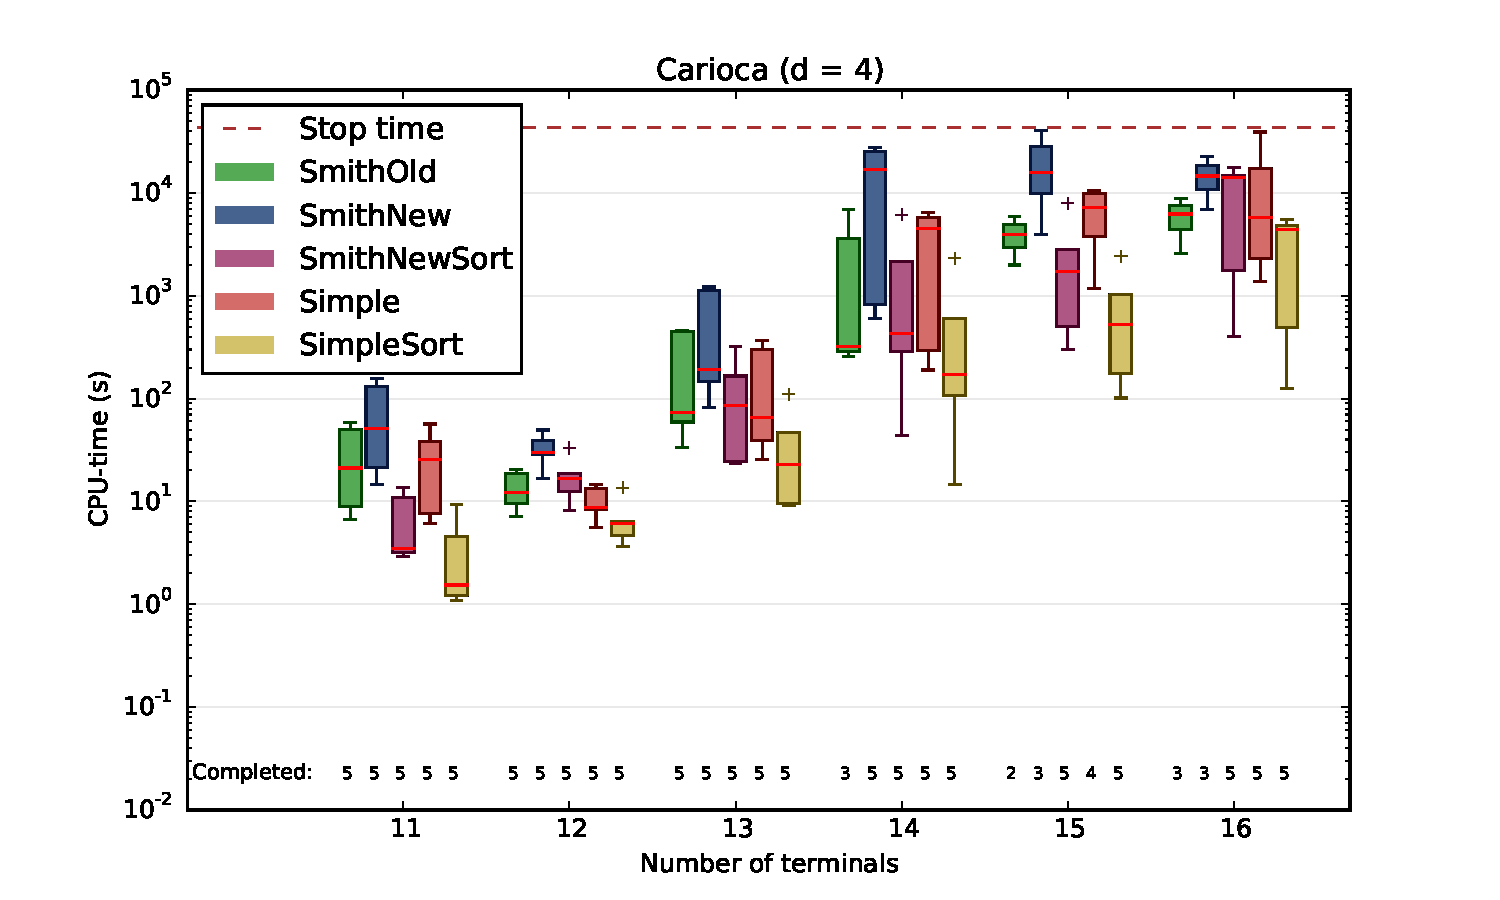
\includegraphics[width=0.8\textwidth]{gfx/boxplots/plot_nvst_boxplot_d4_Carioca_1}
  \caption[Box-plot for Carioca with $d = 4$]{Here be dragons.\label{fig:boxplot-carioca-d4}}
\end{figure}

\begin{figure}[htbp]
  \centering
  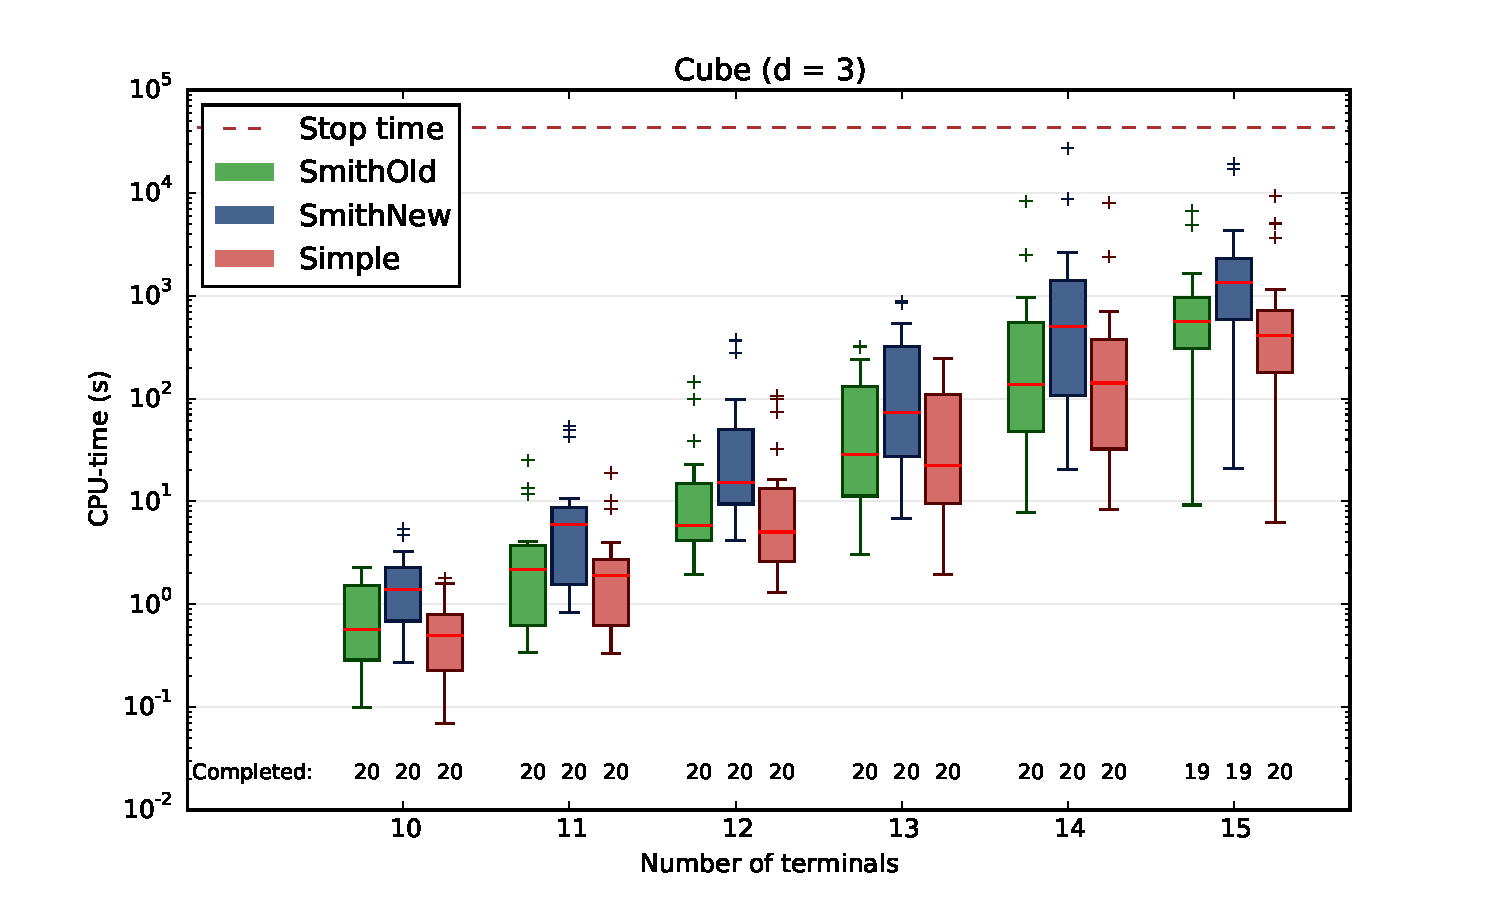
\includegraphics[width=0.8\textwidth]{gfx/boxplots/plot_nvst_boxplot_d3_Cube_1}
  \caption[Box-plot for Cube with $d = 3$]{Here be dragons.\label{fig:boxplot-cube-d3}}
\end{figure}

\begin{figure}[htbp]
  \centering
  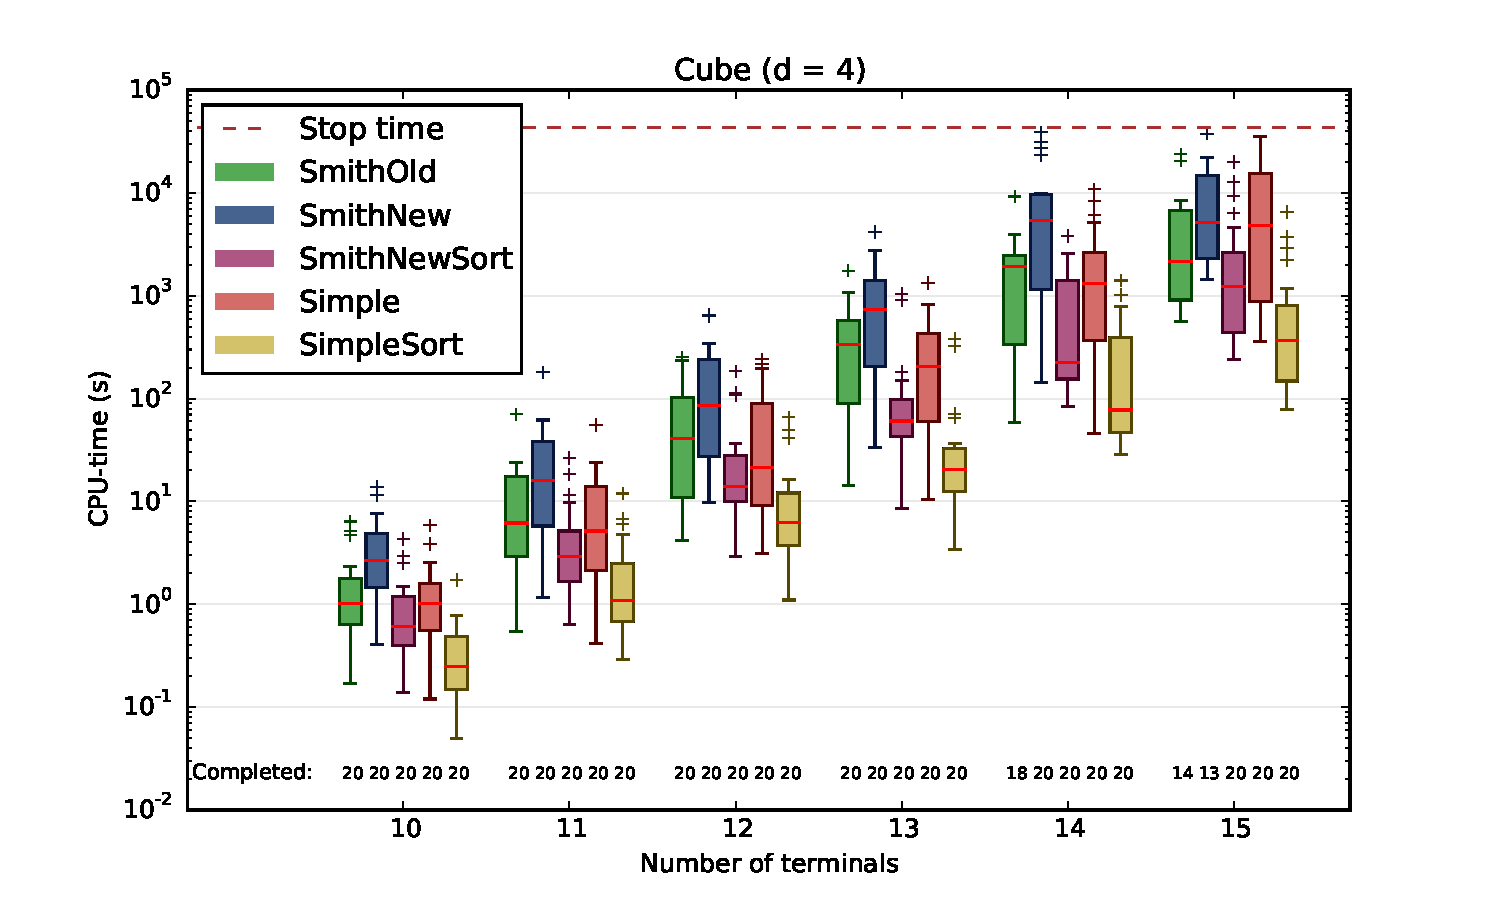
\includegraphics[width=0.8\textwidth]{gfx/boxplots/plot_nvst_boxplot_d4_Cube_1}
  \caption[Box-plot for Cube with $d = 4$]{Here be dragons.\label{fig:boxplot-cube-d4}}
\end{figure}

\begin{figure}[htbp]
  \centering
  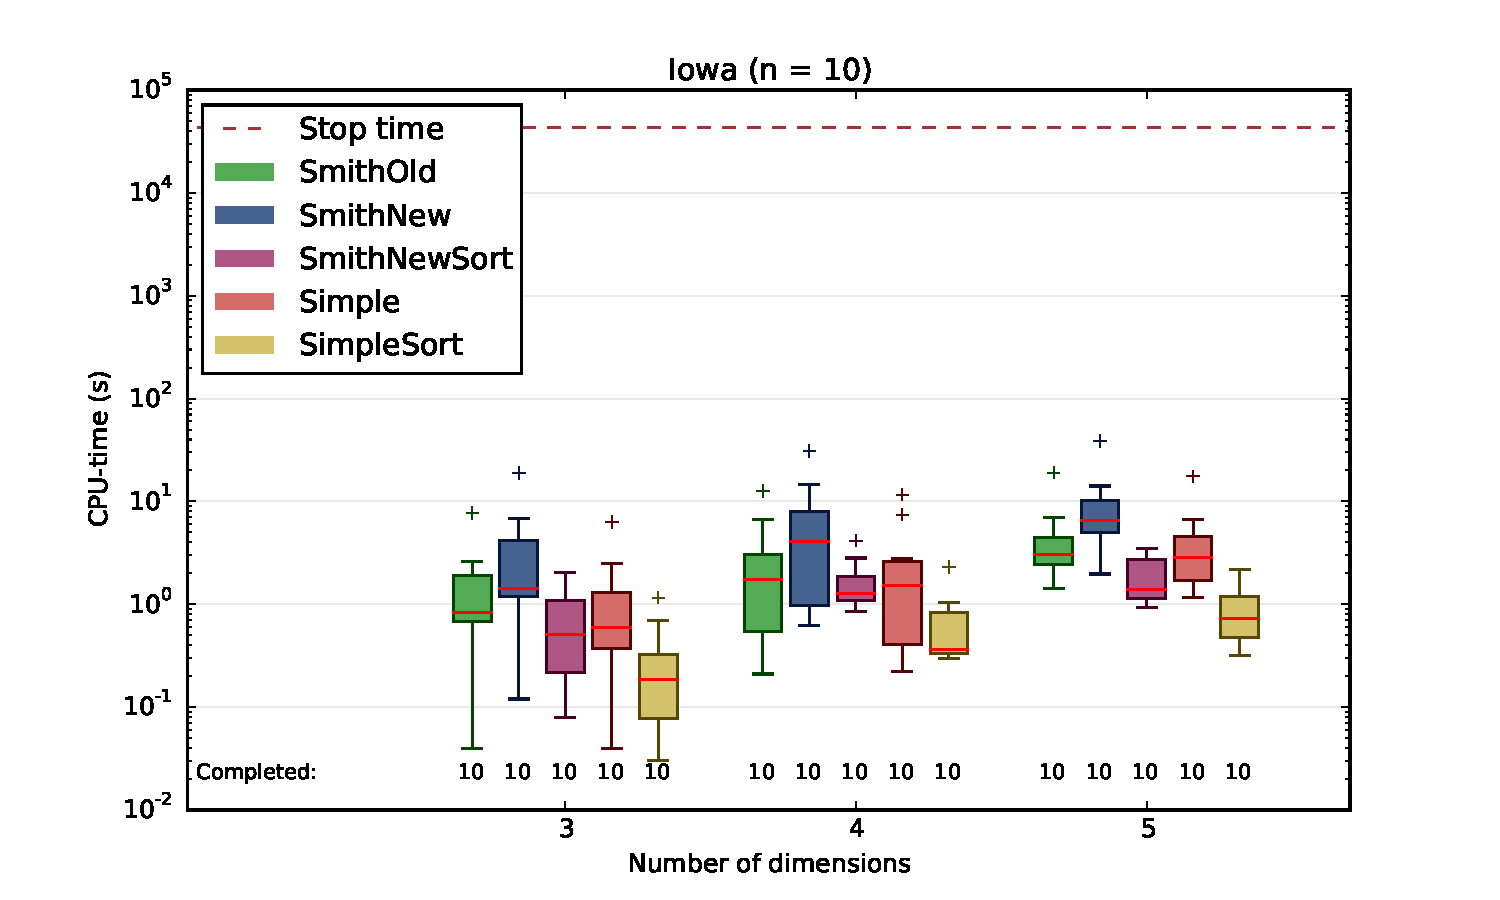
\includegraphics[width=0.8\textwidth]{gfx/boxplots/plot_nvst_boxplot_n10_Iowa_1}
  \caption[Box-plot for Iowa with $n = 10$]{Here be dragons.\label{fig:boxplot-iowa-n10}}
\end{figure}

To compare the speed of the new implementation with the implementation by
\textcite{smith1992} a box-plot of the run times for the Carioca set and Cube
set, where $d = 3$ and $d = 4$, has been plotted in \cref{fig:boxplots-1}. As
can be seen by the two figures the running time of \texttt{SmithNew} is in
general a bit higher than that of \texttt{SmithOld}, whereas the new analytical
solution \texttt{Simple} in general is lower. The reason for the higher running
time of \texttt{SmithNew} is probably due to the fact that the implementation is
done in Go instead of C as the original implementation. Unfortunately we are
therefore not really able to say anything about the performance of the new data
structure for topologies (described in \cref{sec:building-topologies}) being
better of worse than the original implementation. It is however interesting to
see that the analytical solution seems to have better running times than not
only \texttt{SmithNew}, but also \texttt{SmithOld}, as this suggests that an
implementation of this method in a more efficient language, such as C, would
yield even better running times. Further this seems to debunk the claim by
\textcite{smith1992} that a simple iteration would converge slower, at least
speed-wise. Of course we still need to keep in mind the fact that
\texttt{Simple} have showed some sub-optimal trees. It however seems unlikely,
when looking at the percent of sub-optimal results that this should skew the
results so much that this would be changed.

To further compare the effect of sorting the terminals as described
in \cref{sec:sorting-terminals}, box-plots for the Cube set with $d = 3$ and $d
= 4$ has been plotted for \texttt{SmithNew} vs.\ \texttt{SmithNewSort} and
\texttt{Simple} vs.\ \texttt{SimpleSort}. These can be found
in \cref{fig:boxplots-2}. As can be seen from the figures, the run-time of both
methods drop significantly when the terminals are sorted. In almost all cases,
no matter the number of terminals, is the third quartile of the sorted terminals
below the first quartile of the unsorted terminals. The proposed way of sorting
the terminals thus seems to work very well. Also notice, that sorting the
terminals improves the new implementations run-time enough that
\texttt{SmithNewSort} has run-times comparable to/slightly better than
\texttt{SmithOld}.

The reason that the dimensions $d=2$ and $d=5$ have not been plotted is, both
that they show the same situation, but also that $d=2$ is so small that they go
below the graph, and would require another a change of y-axis, and $d=5$ has a
bit to few solved instances for $n=15$ for it to be quite as reliable.

\subsection{Trees and Iterations}
\label{sec:trees-iterations}

Apart from the actual run-time of the implementation, another metric worth
measuring is the number of optimization iterations one runs when solving an
instance, and the number of trees optimized. By the last what is the number of
topology vectors on which we optimize their corresponding tree at least once.

\begin{table}[htbp]
  \centering
    \scalebox{0.8}{
  \begin{tabular}{ccccccc}
    \toprule
         &     & \multicolumn{5}{c}{Method}                 \\
    \cmidrule(l){3-7}
    $n$  & $d$ & \texttt{Simple} & \texttt{SimpleSort} & \texttt{SmithNew} & \texttt{SmithNewSort} & \texttt{SmithOld} \\
    \cmidrule(r){1-2}\cmidrule(l){3-7}
    $10$ & $2$ & $1.04$ & $0.13$ & $1.42$ & $0.17$ & $1.00$ \\
         & $3$ & $1.21$ & $0.25$ & $1.70$ & $0.37$ & $1.00$ \\
         & $4$ & $1.17$ & $0.60$ & $1.61$ & $0.89$ & $1.00$ \\
         & $5$ & $1.54$ & $0.85$ & $2.25$ & $1.34$ & $1.00$ \\
    \cmidrule(r){1-2}
    $11$ & $2$ & $1.05$ & $0.10$ & $1.62$ & $0.13$ & $1.00$ \\
         & $3$ & $1.23$ & $0.19$ & $1.90$ & $0.29$ & $1.00$ \\
         & $4$ & $1.47$ & $0.36$ & $1.97$ & $0.56$ & $1.00$ \\
         & $5$ & $1.54$ & $0.77$ & $2.57$ & $1.22$ & $1.00$ \\
    \cmidrule(r){1-2}
    $12$ & $2$ & $1.17$ & $0.08$ & $1.90$ & $0.11$ & $1.00$ \\
         & $3$ & $1.42$ & $0.16$ & $2.34$ & $0.25$ & $1.00$ \\
         & $4$ & $1.73$ & $0.26$ & $2.83$ & $0.52$ & $1.00$ \\
         & $5$ & $1.53$ & $0.59$ & $2.24$ & $1.11$ & $1.00$ \\
    \cmidrule(r){1-2}
    $13$ & $2$ & $1.11$ & $0.05$ & $2.22$ & $0.09$ & $1.00$ \\
         & $3$ & $1.43$ & $0.12$ & $2.80$ & $0.20$ & $1.00$ \\
         & $4$ & $0.74$ & $0.25$ & $3.19$ & $0.43$ & $1.00$ \\
         & $5$ & $1.66$ & $0.45$ &        & $1.14$ & $1.00$ \\
    \cmidrule(r){1-2}
    $14$ & $2$ & $0.97$ & $0.05$ & $2.63$ & $0.08$ & $1.00$ \\
         & $3$ & $1.61$ & $0.10$ & $3.44$ & $0.19$ & $1.00$ \\
         & $4$ & $1.52$ & $0.16$ &        & $0.39$ & $1.00$ \\
         & $5$ &        &        &        &        &        \\
    \cmidrule(r){1-2}
    $15$ & $2$ & $1.32$ & $0.04$ & $3.12$ & $0.06$ & $1.00$ \\
         & $3$ &        &        &        &        &        \\
         & $4$ &        &        &        &        &        \\
         & $5$ &        &        &        &        &        \\
    \bottomrule
  \end{tabular}
  }

%%% Local Variables:
%%% mode: latex
%%% TeX-master: "../../main"
%%% End:
  \caption[Tree-exploration ratio for Sausage]{The table shows the ratio of
    trees optimized in relation to \texttt{OldSmith}. The number of trees is
    measured such that if a topology vector has been optimized at least once,
    then the number of optimized trees is optimized by one. Topologies that are
    pruned before any optimization has taken place is not counted, and any
    topology can at max be counted once. The data shown are from the Sausage
    set. An empty field means that either the instance for that method, or the
    instance for \texttt{SmithOld} could not be solved within the time
    limit.\label{tab:trees-sausage-ratio}}
\end{table}

\cref{tab:trees-sausage-ratio} shows the number of trees optimized, as a ratio
of the tree optimized by \texttt{SmithOld}, and
\cref{tab:iterations-sausage-ratio} shows the number of iterations, also as a
ratio. Both of these tables are for the Sausage set. As can be seen by the first
table the new implementation, without terminal sorting, optimizes more trees
than the original implementation. Especially \texttt{SmithNew} in some instances
optimizes up to three times as many trees. This is of course not very desirable
and the exact reason for this is unfortunately unknown.

There seems to be several possibilities for the observed behavior. The first
possibility is that the counting of the trees has a bug in either the new or old
implementation, or that it does not count them in the same way. After further
inspection of the source code, this however does not seem to be the case. The
second possibility is that there is a bug somewhere in the new implementation,
causing it to not prune as many trees as the original implementation. This seems
a more likely reason, but inspection of the source code again failed to reveal
such a problem. The third possibility, and probably must realistic, is that the
new data structure for building topologies is at fault. In the original
implementation every new topology vector rebuilds its tree from scratch, meaning
that all Steiner points are replaced---at the perturbed centroid of their
neighbors. However in the new implementation, the Steiner points of the previous
topology is not replaced when splitting the topology and adding another terminal
and Steiner point. It could be thought that as explained in
\cref{sec:correctness} that the error function is faulty, and thus the if-clause
for pruning fails in the new implementation where we may have a initial lower
error for the tree (as most of the tree is already optimized), in contrary to
the old implementation.

As observed with the speed of the program, the number of trees optimized in
general also fails drastically when sorting the terminals (\texttt{SimpleSort}
and \texttt{SmithNewSort}). In all cases the ratio becomes smaller than the
unsorted counter-part, and in most cases it also becomes a lot smaller
\texttt{SmithOld}.

\begin{table}[htbp]
  \centering
  \scalebox{0.8}{
\begin{tabular}{ccccccc}
\toprule
     &     & \multicolumn{5}{c}{Method}                 \\
\cmidrule(l){3-7}
  $n$  & $d$ & \texttt{Simple} & \texttt{SimpleSort} & \texttt{SmithNew} & \texttt{SmithNewSort} & \texttt{SmithOld} \\
\cmidrule(r){1-2}\cmidrule(l){3-7}
$10$ & $2$ & $0.15$ & $0.03$ & $1.10$ & $0.14$ & $1.00$ \\
     & $3$ & $0.23$ & $0.04$ & $1.47$ & $0.28$ & $1.00$ \\
     & $4$ & $0.23$ & $0.08$ & $1.49$ & $0.53$ & $1.00$ \\
     & $5$ & $0.29$ & $0.18$ & $1.37$ & $1.10$ & $1.00$ \\
\cmidrule(r){1-2}
$11$ & $2$ & $0.14$ & $0.02$ & $1.13$ & $0.08$ & $1.00$ \\
     & $3$ & $0.20$ & $0.03$ & $1.57$ & $0.18$ & $1.00$ \\
     & $4$ & $0.24$ & $0.05$ & $1.57$ & $0.32$ & $1.00$ \\
     & $5$ & $0.24$ & $0.08$ & $1.56$ & $0.58$ & $1.00$ \\
\cmidrule(r){1-2}
$12$ & $2$ & $0.14$ & $0.01$ & $1.18$ & $0.06$ & $1.00$ \\
     & $3$ & $0.19$ & $0.02$ & $1.69$ & $0.16$ & $1.00$ \\
     & $4$ & $0.24$ & $0.03$ & $1.67$ & $0.29$ & $1.00$ \\
     & $5$ & $0.22$ & $0.05$ & $1.81$ & $0.40$ & $1.00$ \\
\cmidrule(r){1-2}
$13$ & $2$ & $0.12$ & $0.01$ & $1.23$ & $0.04$ & $1.00$ \\
     & $3$ & $0.17$ & $0.01$ & $1.83$ & $0.12$ & $1.00$ \\
     & $4$ & $0.09$ & $0.03$ & $1.98$ & $0.21$ & $1.00$ \\
     & $5$ & $3.18$ & $0.73$ &        & $8.76$ & $1.00$ \\
\cmidrule(r){1-2}
$14$ & $2$ & $0.09$ & $0.01$ & $1.32$ & $0.03$ & $1.00$ \\
     & $3$ & $0.17$ & $0.01$ & $2.03$ & $0.10$ & $1.00$ \\
     & $4$ & $0.63$ & $0.06$ &        & $0.71$ & $1.00$ \\
     & $5$ &        &        &        &        &        \\
\cmidrule(r){1-2}
$15$ & $2$ & $0.12$ & $0.00$ & $1.42$ & $0.02$ & $1.00$ \\
     & $3$ &        &        &        &        &        \\
     & $4$ &        &        &        &        &        \\
     & $5$ &        &        &        &        &        \\
\bottomrule
\end{tabular}
}

%%% Local Variables:
%%% mode: latex
%%% TeX-master: "../../main"
%%% End:

  \caption[Iteration ratio for Sausage]{The table shows the ratio of iterations
    in relation to \texttt{SmithOld} for the Sausage set. The structure is as
    in \cref{tab:trees-sausage-ratio}. However an iteration means every time we
    perform an optimization, i.e.\ a tree can contribute many times to this if
    we run the iteration for multiple times on the tree (which we most likely
    do).\label{tab:iterations-sausage-ratio}}
\end{table}

Looking at the second table (showing the iteration ratios) we see more or less
the same situation, as in the first table. However a column which is interesting
is the one for \texttt{Simple}. As can be seen in the first table, the ratio for
the number of optimized trees in general is slightly above $1$. However the
ratio for iterations is in general below $0.5$. This means that \texttt{Simple},
is a lot quicker at reaching a low error and thus stopping to optimize the
trees. This should mean that the analytical solution converges a lot faster than
\autocite{smith1992}'s iteration. However again we need to remember the results
from \cref{sec:correctness}, which means that we need to be a bit cautious with
such a conclusion. However again the ratio is consistently lower for the number
of iterations\footnote{Except for a single outlier}, and thus is seems unlikely
that the result is solely due to sub-optimality, as described earlier.

A thing worth noticing is that the higher run-times observed in the previous
section makes a lot more sense when observing the ratios for trees and iterations.
Thus it is very possible, that if the source of this could be identified, that
the new implementation would have faster run-times than \texttt{SmithOld} all around.

%%% Local Variables:
%%% mode: latex
%%% TeX-master: "../../main"
%%% End:
